\chapter{Introduzione}
\label{cap:intro}

Nella guida automatizzata, le mappe digitali completano i sensori delle auto. Utilizzando i dati della mappa, il sistema di guida automatizzata può anticipare la strada da percorrere, vedendo ben oltre la gamma dei sensori del veicolo. Il risultato è un veicolo in grado di vedere dietro gli angoli e di adattare il suo comportamento alla guida in condizioni di scarsa visibilità come pioggia o nebbia. La fusione di dati provenienti da diversi sensori con le  informazioni aggiunte dalle mappe digitali rende la guida automatizzata più sicura e precisa, poiché il sistema può gestire circostanze più estreme e aggiunge ridondanza.
\begin{figure}[H]
        \begin{center}
            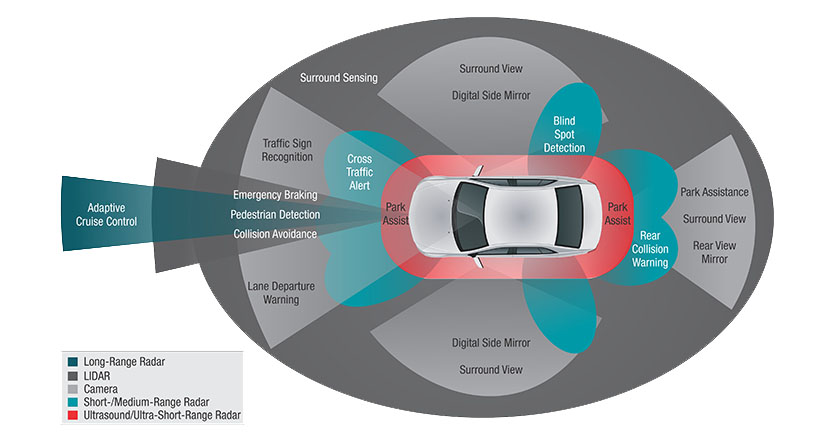
\includegraphics[width=0.7\textwidth]{Immagini/adas.jpg}
        \end{center}
    \caption{ADAS}
\label{fig:ADAS}
\end{figure}

Dal controllo adattivo della velocità di crociera (ACC) all'assistenza autostradale, fino alla guida autonoma (AD), beneficiano tutti di vari livelli di granularità forniti dalle mappe. Maggiore è il livello di autonomia del veicolo (\ref{fig:SEA}), più requisiti devono soddisfare le mappe digitali.

\begin{figure}[H]
        \centering
        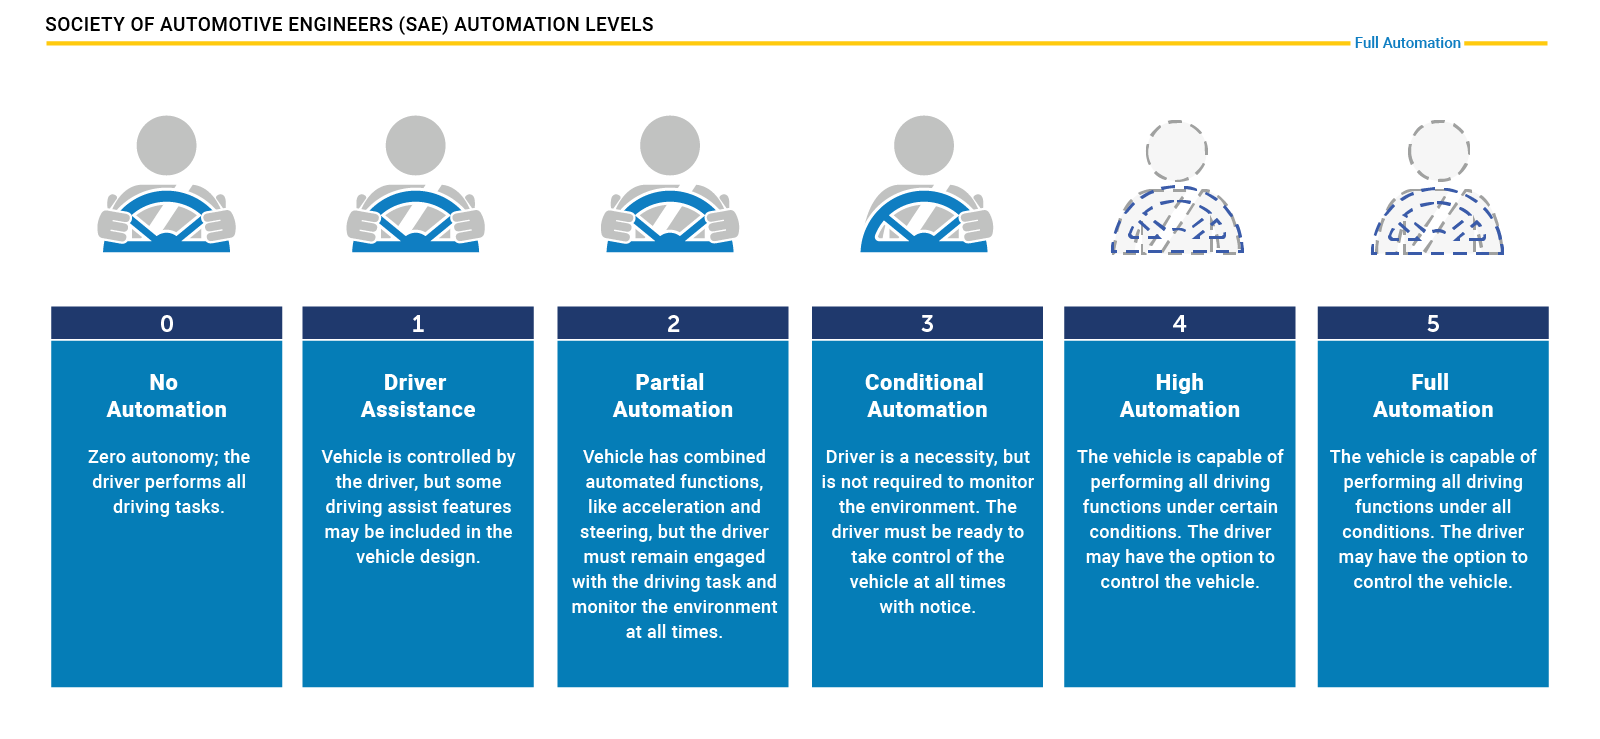
\includegraphics[width=1.1\textwidth]{Immagini/levels.png}
        \caption{livelli di automatizzazione veicoli definiti dalla SEA.}
        \label{fig:SEA}
    \end{figure}

Per soddisfare questi casi d'uso, esistono due tipi di mappe specializzate per la guida assistita e automatizzata: la mappa ADAS e le mappe HD a copertura ridotta, ma a più alta precisione.

\subsection*{Mappe ADAS}
I veicoli che rientrano nei livelli 1 e 2 di automazione utilizzano le mappe ADAS per l'assistenza al guidatore e gli avvisi di sicurezza ad esempio per il line assist o per il controllo di velocità adattivo, esse sono quindi utilizzate per avere una guida più sicura e confortevole.

\subsection*{Mappe HD}
Quando si passa dalla guida assistita alla piena autonomia, ovvero ai Livelli 2, 3 e oltre, la mappa HD diventa la soluzione migliore per una guida autonoma sicura. Sebbene estremamente accurate, le mappe ADAS raggiungono il loro limite quando sono richiesti maggiore precisione e livello di dettaglio.
Le mappe HD invece aumentano la precisione a risoluzioni di pochi centimetri. Utilizzando informazioni dettagliate come limiti di velocità a livello di corsia, oggetti statici ad esempio segnali stradali e arredi stradali, edifici e geometria della corsia, le mappe HD consentono ai veicoli automatizzati e autonomi di diventare context-aware, ovvero di aver informazioni dettagliate rispetto alla loro posizione, all'ambiente e al percorso da seguire.

\section*{Obiettivi}
Lo scopo di questo lavoro è di creare una pipeline in grado di inserire all'interno delle mappe di OpenStreetMap point cloud che descrivono le faciate degli edifici e in seguito poterle recuperare in modo da aumentare il grado di informazione disponibile, affinchè le informazioni aggiunte possano essere utilizzate per migliorare la localizzazione del veicolo sulla corsia, il risultato verrà infatti processato dal sistema \textit{Road Layout Estimation} (RLE) sviluppato all'interno del laboratorio IRA dell'Università di Milano-Bicocca, in particolare dal componente \textit{Building Detector}\cite{7795618}, per cercare di fornire un' ipotesi di localizzazione più accurata rispetto alla scena percepita da un veicolo.
Il diagramma di flusso seguente descrive il lavoro che è stato sviluppato:

\begin{figure}[H]
    \centering
    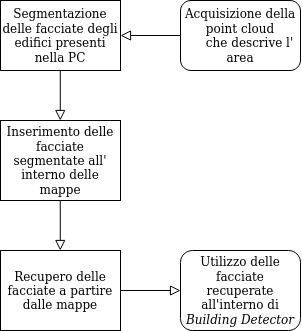
\includegraphics[width=0.5\textwidth]{Immagini/Pipeline.png}
    \caption{Pipeline implementata}
    \label{fig:Pipeline}
\end{figure}

Il progetto consiste quindi in tre parti ben distinte ma ciascuna necessaria per ottenere il risultato finale:
\begin{enumerate}
    \item La definizione di una algoritmo di computer vision che permetta di segmentare le singole facciate degli edifici che possano essere utilizzate dalla seconda parte.
    \item La modifica delle mappe per integrare i dati aggiunti e la messa in opera di un servizio web che metta a disposizione le mappe modificate.
    \item La creazione di un servizio in grado di scaricare e mettere a disposizione le facciate integrate all'interno delle mappe.
\end{enumerate}{}
Nel primo capitolo è stato utilizzato \hyperref[sez:PCL]{PCL} per scrivere l'algoritmo di segmentazione degli edifici attraverso opportuni filtraggi effettuati sulla point cloud in ingresso.\\

Nella secondo capitolo è stato utilizzato \hyperref[sez:Docker]{Docker} e le api di \hyperref[sez:OSM]{OSM} per poter mettere a disposizione le mappe modificate con l'inclusione delle point cloud delle facciate.\\

Nella terzo capitolo invece si è interagito con \hyperref[sez:RLE]{RLE} e si è quindi utilizzato \hyperref[sez:ROS]{ROS} per poter scrivere un servizio di retrival delle point cloud.\\ 
Ogni parte sarà trattata in modo più approfondito nei rispettivi capitoli.

\section*{Dataset}
I dati utilizzati per testare questo progetto di tesi sono messi a disposizione dal KAIST Urban Dataset\cite{jeong2019complex}.
Questo dataset fornisce dati LiDAR (Light Detection and Ranging) e immagini stereo uniti a vari sensori di posizione che descrivono un ambiente urbano molto complesso, vengono forniti i dati di LiDAR 2D e 3D, e i dati che descrivono la navigazione del veicolo. Per comodità, gli strumenti di sviluppo sono forniti nell'ambiente Robot Operating System (ROS).

\subsection*{Sistema di acquisizione}
La piattaforma utilizzata per acquisire i dati dei sensori è una Toyota Prius (\ref{fig:SystemCar}). Il veicolo è dotato di due LiDAR 2D e due 3D per raccogliere dati sull'ambiente circostante. Il 3D LiDAR è stato montato con un angolo di 45 gradi per la massima copertura. Nel caso del LiDAR 2D, il sensore posteriore è stato collocato verso il basso per informazioni sulla strada e il sensore anteriore è invece direzionato verso l'alto per informazioni sugli edifici. La telecamera stereo è stata installata di fronte alla parte anteriore del veicolo. (\ref{fig:SystemSensors})
Inoltre, sono stati collocati vari sensori per stimare la posizione del veicolo. GPS e VRS GPS sono stati installati per stimare la posizione globale. Il GPS consente di immagazzinare informazioni generiche sulla posizione, al contrario il VRS GPS stima accuratamente la posizione del veicolo. Inertial Measurement Unit (IMU) e Fibre Optic Gyro (FOG) sono stati montati per misurare l'odometria del veicolo. L'IMU è un sensore che restituisce informazioni approssimative, il FOG fornisce invece valori estremamente più precisi rispetto all'IMU. Tutte le informazioni sui sensori sono fornite in formato raw con un timestamp.
Prima del loro utilizzo i dati acquisiti sono stati fusi con uno script sviluppato all'interno del laboratorio IRA in un unica mappa contenente tutti i valori provenienti dai sensori.

\begin{figure}[H]
    \centering
    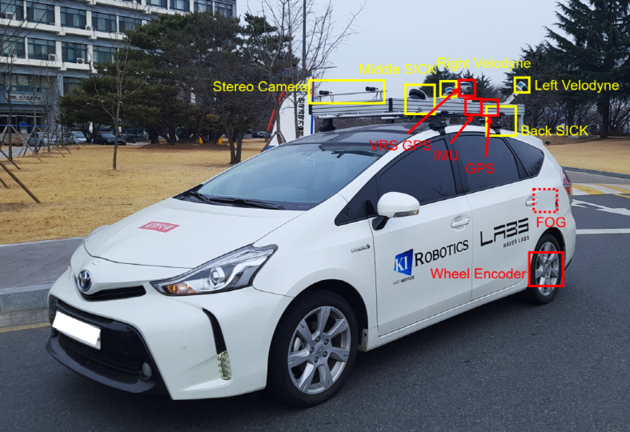
\includegraphics[width=0.8\textwidth]{Immagini/system_car.png}
    \caption{Auto utilizzata per acquisire i dati}
    \label{fig:SystemCar}
\end{figure}

\begin{figure}[H]
    \centering
    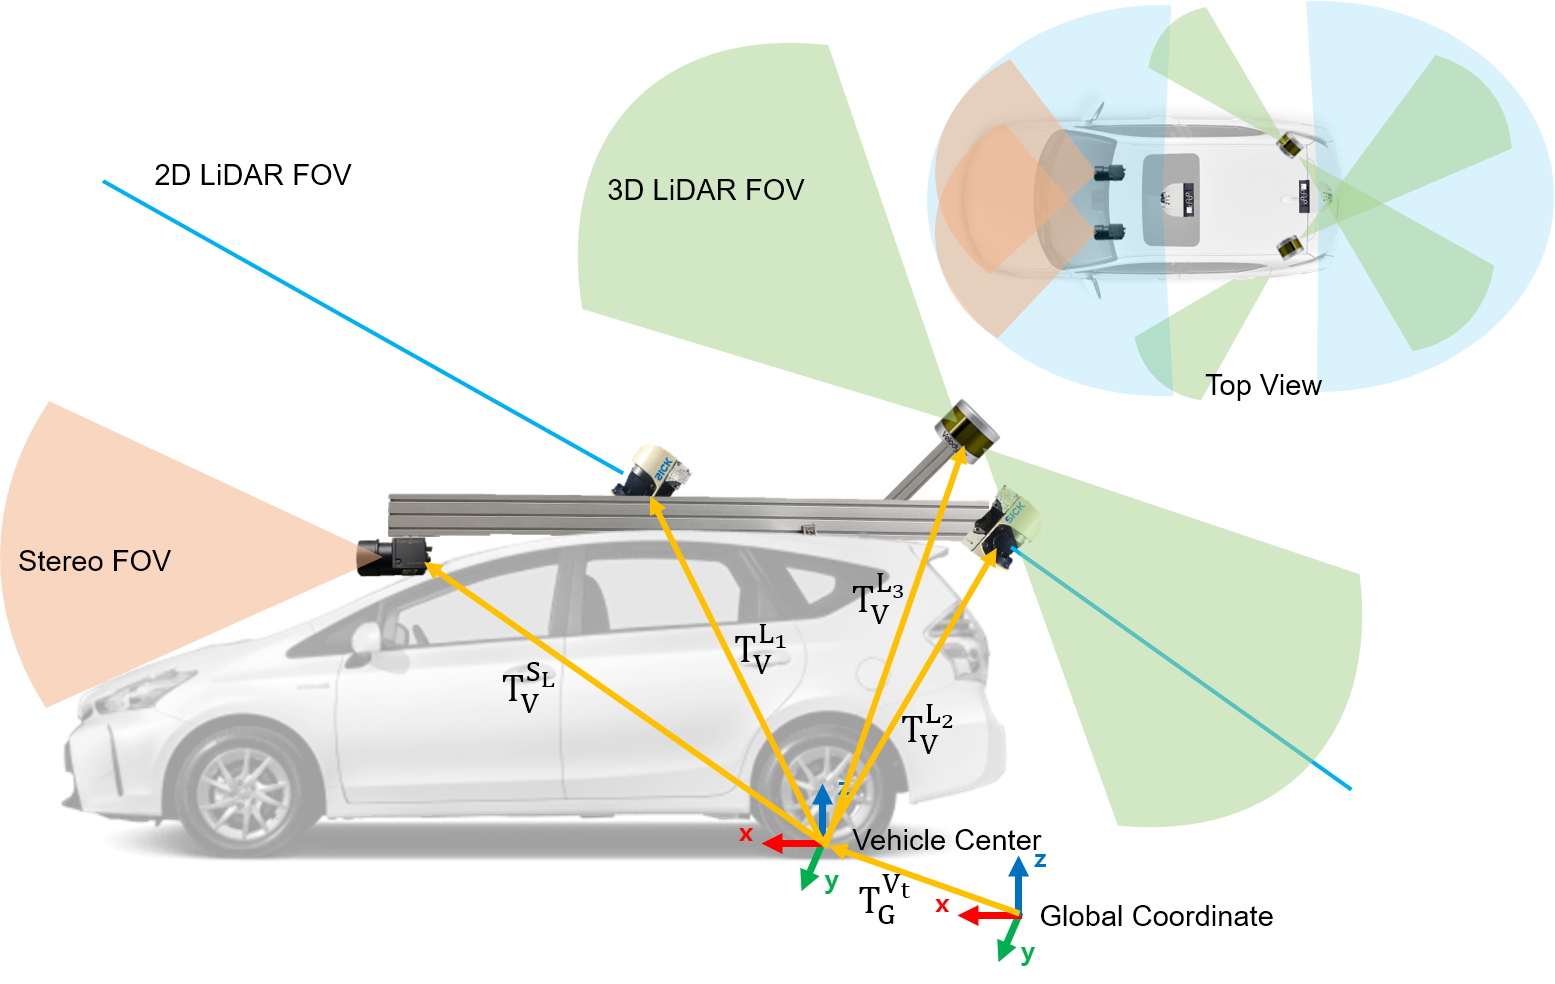
\includegraphics[width=0.8\textwidth]{Immagini/system_sideview.png}
    \caption{Vista dettagliata dei sensori utilizzati per acquisire i dati}
    \label{fig:SystemSensors}
\end{figure}
\newpage

